
\documentclass[a4paper,twoside,notitlepage,11pt]{article}
\usepackage{graphicx}
\usepackage{hyperref}
\usepackage{amstext}
\usepackage{tabularx}
\usepackage{amssymb}
\usepackage{fancyhdr}
\usepackage{setspace}
\usepackage{fancyvrb}
\usepackage[all]{xy}
\usepackage{stmaryrd}
\usepackage{nccmath}
\usepackage[a4paper,hmargin=50pt,vmargin=75pt]{geometry}
\usepackage[hypcap]{caption}
\usepackage{qtree}
\usepackage{cleveref}
\usepackage[normalem]{ulem}
\usepackage{float}
\usepackage{layouts}
\usepackage{wrapfig}
\usepackage{listings}
\usepackage{color}
\usepackage{mathpartir}
\usepackage{fancyeq}
\usepackage{menukeys}

\newcommand{\paperTitle}{Niceway.to Design Specification}
\newcommand{\from}{\leftarrow}

\pagestyle{empty}
\renewcommand{\headrulewidth}{0.0pt}

\fancypagestyle{plain}{
\fancyhf{}
\fancyhead[LE]{\thepage}
\fancyhead[CE]{\textit{\paperTitle}}
\fancyhead[RE]{Craig Knott}
\fancyhead[LO]{Craig Knott}
\fancyhead[CO]{\textit{\paperTitle}}
\fancyhead[RO]{\thepage}
}

\begin{document}

\begin{center}
 \ \\[4cm]
 {\LARGE \textbf{\paperTitle} \\ [0.2cm]}
   \textbf{Craig Knott} \\
    \textbf{Version 1.0}\\
	 \textbf{\today}
\end{center}

 \tableofcontents
  \newpage
   \pagestyle{plain}
 
 \section{Requirements}
 \subsection{Functional Requirements}
 \begin{enumerate}
 \item[1.] The user should be able to search by geographic region and discover submitted routes for that region.
 \item[2.] The user should be able to contribute routes.
 	\begin{enumerate}
 	\item[2.1.] Only the creating user should be able to modify these routes
 	\item[2.2.] The user should be able to decide on the visibility of this route (private or public)
 	\end{enumerate}
 \item[3.] The user should be able to interact socially with the route, including:
 	\begin{enumerate}
 	\item[3.1.] Comment on public routes
 	\item[3.2.] Recommend alternative routes
 	\item[3.3.] Share routes to external social media websites
 	\end{enumerate}
 \item[4.] Users should be able to create accounts and specify for example, name, age, email and location 
 \item[5.] The should be administrative users who have extra functionality available, including:
	 \begin{enumerate}
 		\item[5.1.] Manage users
 		\begin{enumerate}
 			\item[5.1.1.] Delete users
 			\item[5.1.2.] Update users
 			\item[5.1.3.] Create users
 		\end{enumerate}
 		\item[5.2.] Manage routes
 		\begin{enumerate}
 			\item[5.2.1.] Delete routes
 			\item[5.2.2.] Update routes
 		\end{enumerate}
 		\item[5.3.] Moderate comments
 		\begin{enumerate}
 			\item[5.3.1.] Delete comments
			\item[5.3.2.] Update comments
 		\end{enumerate}
 		\item[5.4.] Make announcements
 		\item[5.5.] Make backups of the website in a standard, compliant, free and open format
 		\item[5.6.] De-authorize active sessions
 		\item[5.7.] Lock the site and prevent access
 	\end{enumerate}
 \item[6.] Users should be able to export their routes to a FOSS
 \item[7.] Users should be able to fork other user's public routes (make a copy), and edit as they wish
 \item[8.] There should be a route editor component which allows the user's to create and specify their route
 \item[9.] The user should be able to log into their account and:
	 \begin{enumerate}
	 	\item[9.1.] Access and change personal information
	  	\item[9.2.] Access and edit their submitted routes
	 \end{enumerate}
 \end{enumerate}
 
 
 \subsection{Non-Functional Requirements}

\paragraph{Accessibility}\ \\
The proposed system is to be made available entirely on-line, allowing anyone with internet access, and a computer, to use the system. As the application will be web-based, the user is not required to download anything to start using it, this will make it more accessible for the user, and it will be easier for them to get started using the application. The only potential issue with a web-based application is if the server goes down, or if the domain expires. The server going down does not, unfortunately, have a solution, but keeping the domain should be relatively trivial.

\paragraph{Usability and Operability}\ \\
The project should be designed in such a way that users ranging from a low level of skill, to a high level of skill should be able to use it with little prior knowledge. There will be a dedicated help system present in the system, that will allow the user to get help, whenever they need it, without having to leave the system and check some external documentation. The project will be developed as a fully-responsive web application, meaning mobile devices will be fully supported.

\paragraph{Maintainability \& Documentation}\ \\
The system must be exceptionally well documented allowing for easy maintenance by an external developer. This includes both an easy to understand code structure, as well as commented code (specifically using JSDoc), which should be kept as modular as possible.  The system itself will have help available to the user, so that if they are confused, they can be guided in the right direction.

\paragraph{Quality}\ \\
As this system is to be used externally, and will be a representation of both myself, and the client, there are several quality issues that must be addressed. The system must be built so that it is robust, and works as the user expects, but it must also contain as few bugs as possible. Any bugs that are identified should be reportable to the maintainer, and be fixed as soon as possible.\ \\
\ \\
The quality of the code must also be considered. In this regard, the code will be written in as modular a way as possible, and useful comments will be provided to highlight the purpose of each function, and to illustrate any particularly complex code.

\paragraph{Resource Requirements and Constraints}\ \\
As this system is aimed at users with a mixture of skill levels, no assumptions can be made on the level of hardware that the users will possess. For this reason, the system will be designed to use as few resources as possible. Fortunately, due to being a web-based system, the load of the system would be fairly minimal anyway, as it is mostly loading only JavaScript and HTML 5. The only true computation takes place on the server, and thus would not be a concern for the user.\ \\
\ \\
The ability to load and save files potentially causes a problem, but only if the user has very little hard drive space, and attempts to save an extremely large file from the system. Unfortunately, there is nothing that can be done about this, although even very large systems will have a relatively small file size.\ \\
\ \\
The final concern is internet bandwidth which, whilst not a problem on desktops, will be a problem for mobile phones. This is why the amount of data sent to the user when they are navigating a route will be kept to a minimum, so that they do not use up their data allowance (or drain their battery).

\paragraph{Cross Platform Compatibility}\ \\
Due to the project being a web-based system (developed using HTML5, CSS3, and JavaScript), it is difficult for it not to be cross platform compatible. However, there are still a few issues that may have to be dealt with, especially when looking at different browsers that the user may be using. For this reason, research into how the system performs on different browsers will be important, so that it can be assured that any user using any browser will have full access to the system, as it was meant to be.

\paragraph{Security}\ \\
Security is a concern for this project, as the user's will be able to create accounts with the system, and therefore their data will need to be stored. This data will be stored in compliance with the Data Protection Act, and all passwords will be encrypted. Cookies may also be utilised on the site, so a cookie disclaimer will also be necessary. 

\paragraph{Disaster Recovery}\ \\
 The administrator should be able to take backups of the site in a standard, compliant, free and open format. They should also be able to de-authorize active sessions, and lock the website to prevent access. As far as the code base itself, the project will be stored both on the server, and in a Git repository, allowing for recovery if anything goes wrong.
\newpage 
\section{Annotated Designs}
In this section, three potential designs for each of the main pages of the application have been included, as well as annotations which link design decisions to the functional requirements. These designs focus on the landing page (which doubles as the route discovery page), the route creation page, the route listing page, and a single design for the route creation page. The other pages of the application are simple form pages, and do not need much thought, thus they have been included separately in section \ref{subsec:gpd}, along with some annotations. 

\subsection{The Landing Page/Route Discovery Page}
The purpose of the landing page (which doubles as the route discovery page), is to allow the user's for look for routes they may be interested. This is achieved by some search functionality, with the ability to specify extra filters if the user wishes (FR 1). 

\paragraph{Minimal Design}\ \\
The main driving idea behind the first design, is simplicity. It should be clear to the user, at all points, what they can do and what their next steps should be. This design sports a large map which, if possible, displays the user's current location in the background. This helps the user feel more acquainted with the application, because it is showing familiar surroundings - this is also the reason for displaying the ``Welcome, \textit{name}'' message by the search bar (although it will show ``explorer'' instead of the user's name if they are not logged in).\ \\
\ \\
To keep the page looking as clean as possible, the extra filter options are initially hidden (this includes price of petrol, distance travel, etc). This means users are able to search for routes, without being bombarded with a large number of form elements. This clean design and low number of elements on the page, make it very easy for the user to identify what this page's purpose is - searching for routes.
\begin{figure}[!ht]
\vspace{6mm}
 \begin{center}
		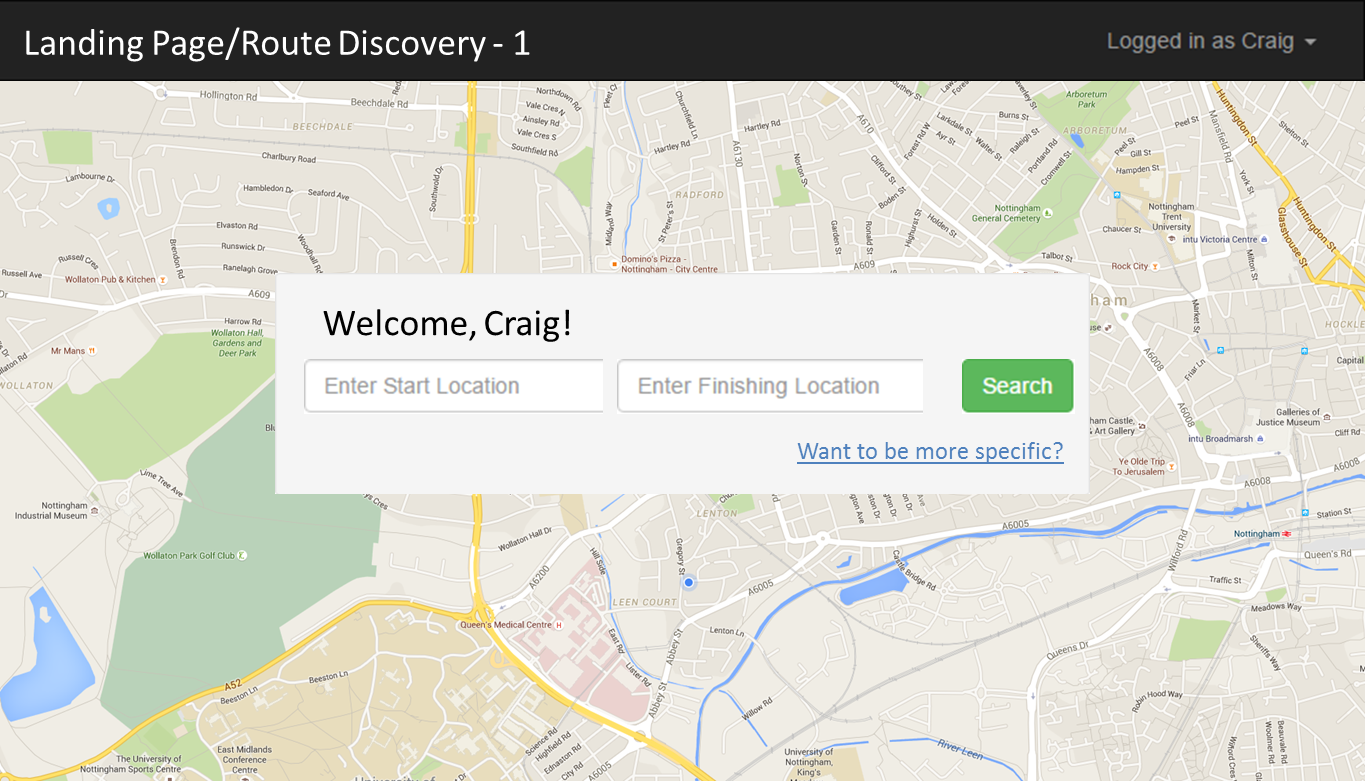
\includegraphics[width=0.8\textwidth]{images/ui-landing-1.png}
	\end{center}
	\vspace{-6mm}
\end{figure}\ \\

\newpage 
\paragraph{Detailed Search Design}\ \\
Compared to the first design, this design is less minimalistic, as it has all searchable fields visible on the page at once. There is an issue here that the users see this large number of fields and are intimidated and exit the application. To combat this it has been placed on the left hand side - this allows the users to view the site from left to right, as would be expected, and thus more comforting. This also gives the map a large interrupted view, which is aesthetically pleasing to look at.\ \\
\ \\
The design ties in well with design 2 of the route listing page, which displays all the search results in the left hand side of the screen. This would mean that the UI could update slightly to display the search results, and the route listing page would be visible without requiring a new page to be loaded - speeding up the process.
\begin{figure}[!ht]
	\begin{center}
		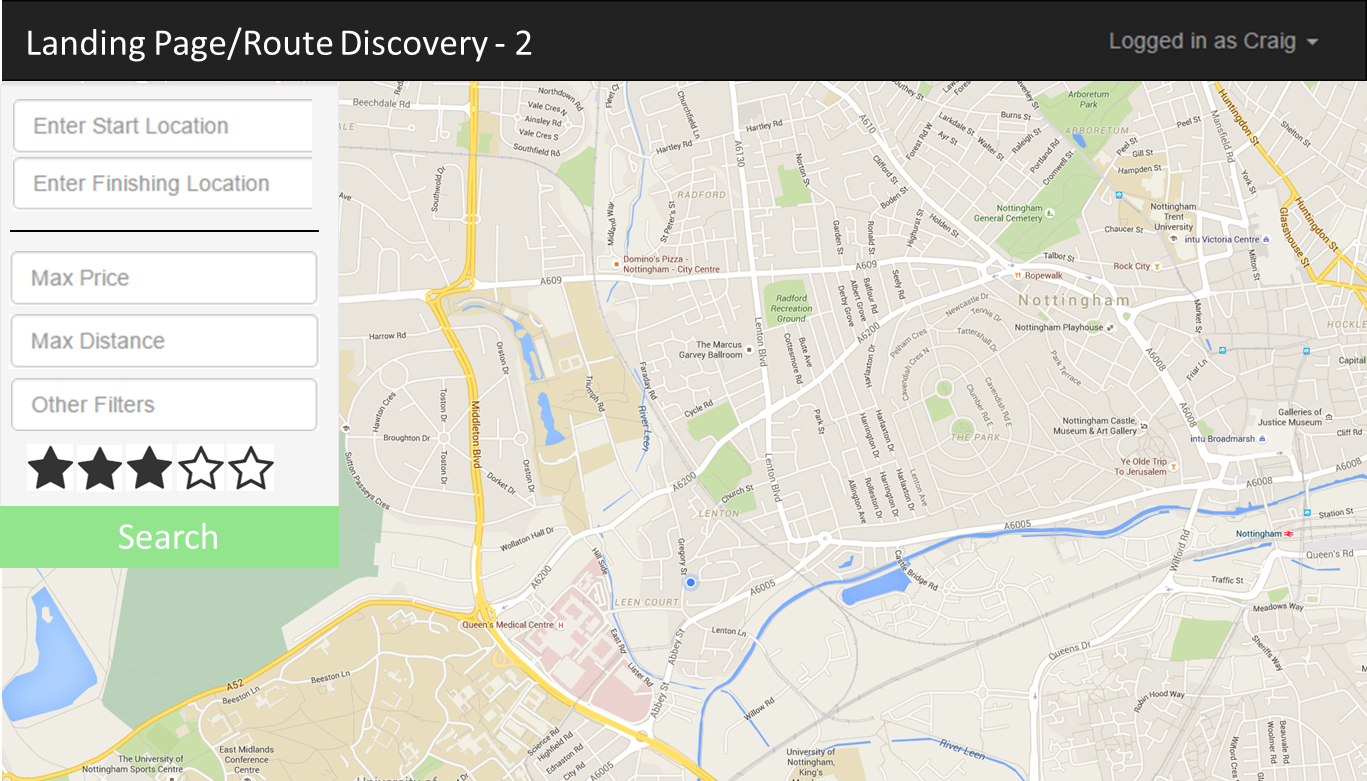
\includegraphics[width=0.70\textwidth]{images/ui-landing-2.png}
	\end{center}
	\vspace{-9mm}
\end{figure}

\paragraph{Modern Design}\ \\
The third design was slightly more unique, and would be supplemented with CSS animations to make it more modern looking. The aim of this design is to look modern, and split up data entry, so that the user is not overwhelmed. They are able to enter the start and end location and then, based on that, enter filtering options. This help to reduce the individual cognitive load of each of the steps, but means that there are more steps to go through until the user reaches the route detail page. Another issue to consider is that the user may be initially lured in by only requiring to enter two fields, but feel cheated when they are then presented with several more.


\begin{figure}[!ht]
	\begin{center}
		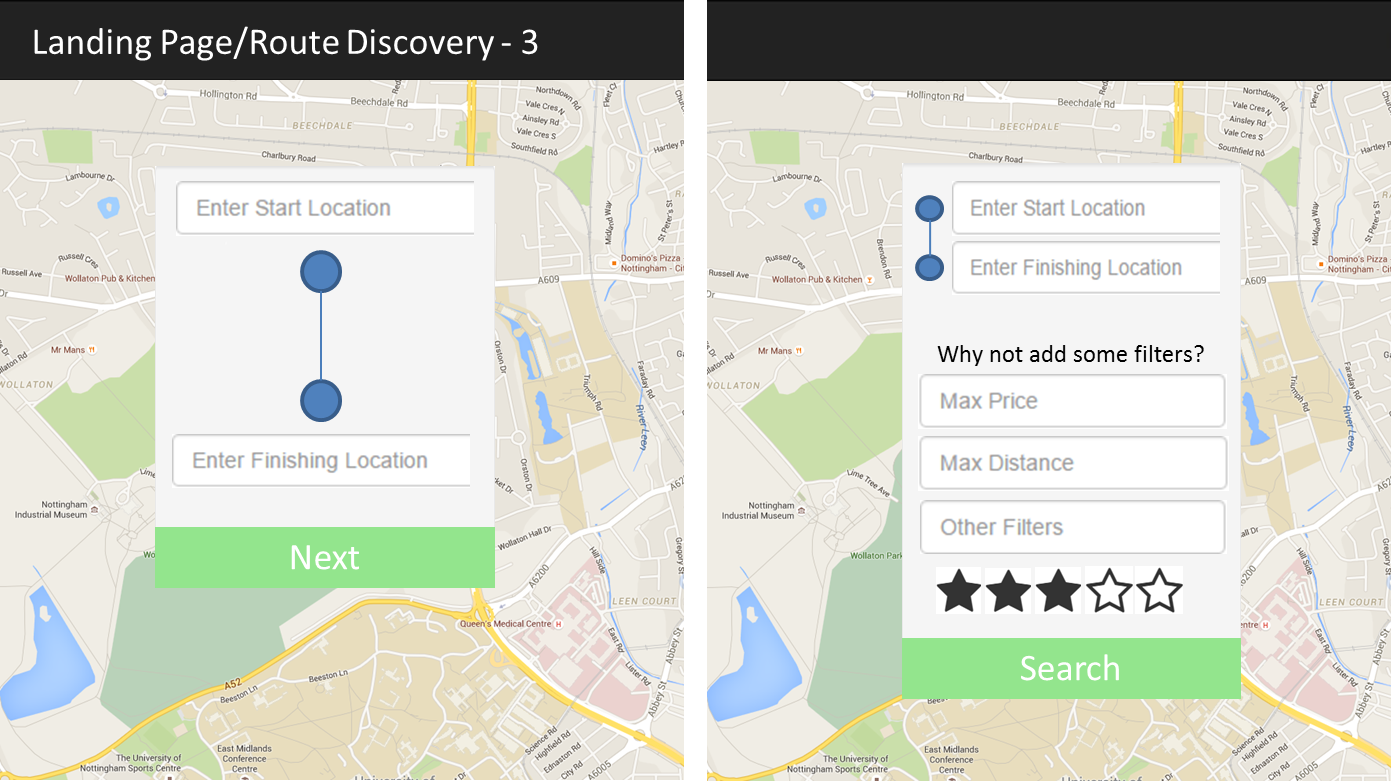
\includegraphics[width=0.70\textwidth]{images/ui-landing-3.png}
	\end{center}
	\vspace{-10mm}
\end{figure}


\newpage 

\subsection{The Route Listing Page (RLP)}
The purpose of the route listing page was to display all of the routes that satisfied the user's search criteria, from the route discovery page. It is important that as many routes are shown as possible (to increase diversity, and the number of choices available), and that they are displayed in a clear, and easy to digest format. (FR 1).

\paragraph{Two Column Design}\ \\
The first design sports a large map, and a clear separation between the map and the list of routes. This dual layout meant that users could find a route in multiple ways - they could select a route from the list that caught their eye, or they could select a route that was close to a specific location (from the map view). This freedom helps to prevent the user becoming confused, or frustrated, when they cannot achieve their goal. The map view is also useful for identifying related routes, which could entice the user to visit the application again later.\ \\
\ \\
The main drawback of this design is the vast quantity of information displayed to the user at once. There is the list, which is a large amount of textual data, combined with the map, which is a large amount of image data. This vast choice could overwhelm the user, and they may not be able to pinpoint any route the would like to traverse. There is also a potential problem in that, if there are a huge number of routes, the map could become cluttered and unusable.
\begin{figure}[!ht]
\vspace{6mm}
	\begin{center}
		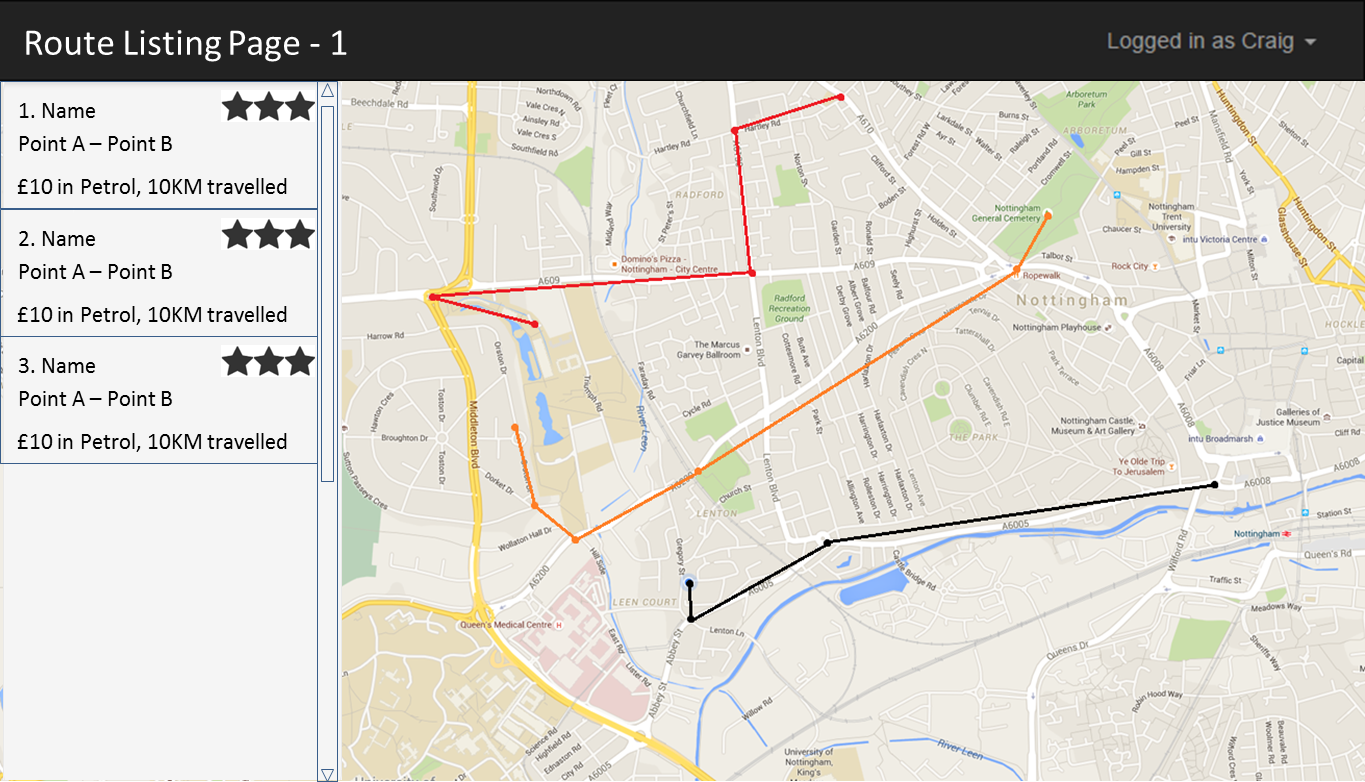
\includegraphics[width=0.85\textwidth]{images/ui-rlp-1.png}
	\end{center}
	\vspace{-6mm}
\end{figure}

\newpage 
\paragraph{Minimalist Design}\ \\
This design also featured a large map. In fact, this map was even larger than the map present in the first design. This is because this design did not feature a textual listing of the routes available. Instead, it relied solely on the graphical display of the routes to provide the user interaction. This makes the design very minimalistic and simple, but a novice user could easily be confused as to what they had to do at this step, and give up (admittedly it would not be too difficult to add a simple pop-up that explained the page). The terms that were used whilst searching for these routes are displayed as pills at the top of the page, so the user can identify if they have made any mistakes in their search.

\begin{figure}[!ht]
	\begin{center}
		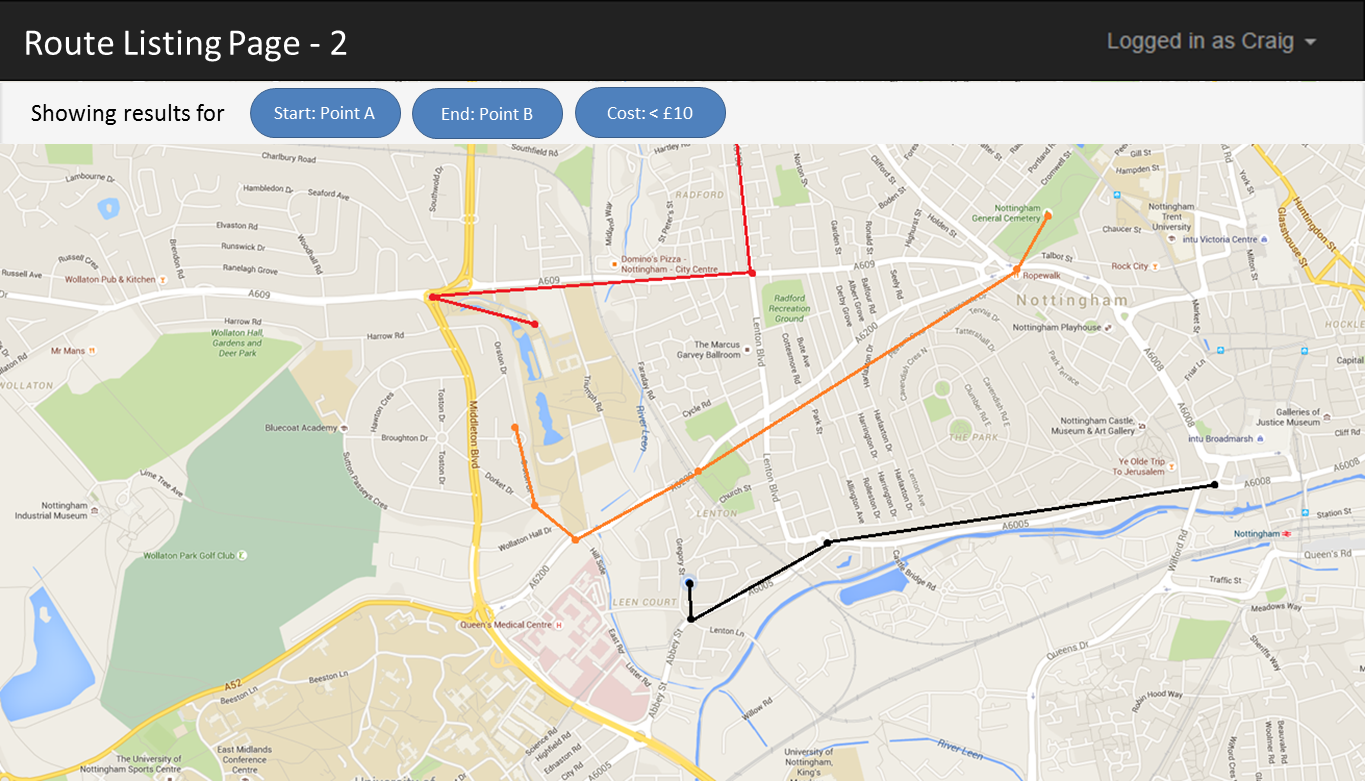
\includegraphics[width=0.7\textwidth]{images/ui-rlp-2.png}
	\end{center}
	\vspace{-9mm}
\end{figure}

\paragraph{Map-less Design}\ \\
The final design for the route listing page differed from the others in that it didn't display one large map with all of the routes. Instead, it opted to show each of the routes individually on their own map. This meant that each one could be considered separately, and the user wasn't overwhelmed with a huge variety of routes at once. The other key feature of this design was the inclusion of the discovery UI. This meant that the user could search again directly from this page, instead of needing to go back to the landing page, like that would in the other designs.\ \\
\ \\
The main problem of this design is that, if there are many routes, those at the bottom of the list would never be seen, as the user probably would not scroll that far. To combat this, some randomness could be added to the algorithm that determines the order of the routes. However, this would also encourage submissions to be of a higher quality, so that they were not placed far down in the list.
\begin{figure}[!ht]
	\begin{center}
		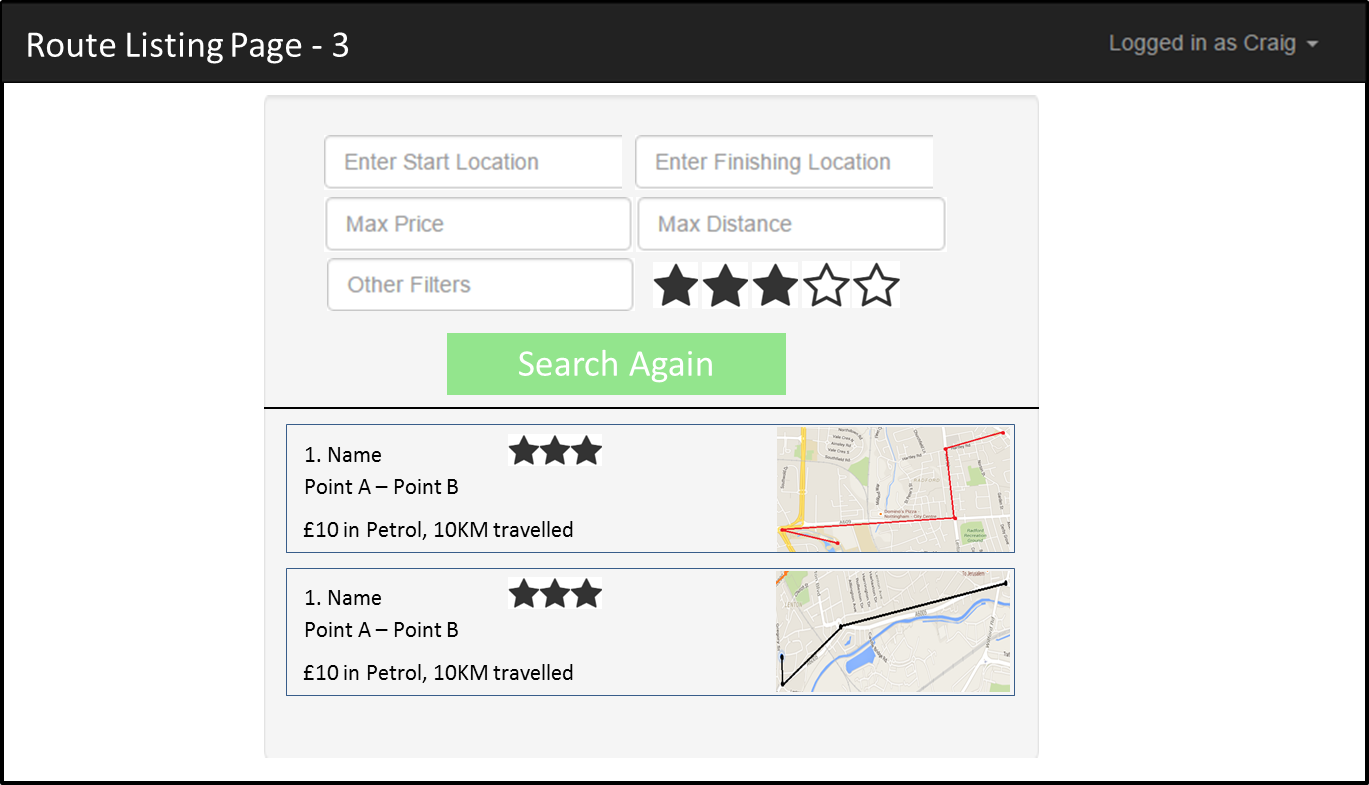
\includegraphics[width=0.7\textwidth]{images/ui-rlp-3.png}
	\end{center}
	\vspace{-9mm}
\end{figure}

\subsection{The Route Detail Page (RDP)}
The purpose of the route detail page is to display both the route, and meta information about it. It is important that information on this page is easily accessible, so users can make informed decisions as to whether or not they wish to travel a route or not. Users will also be able to see, and leave comments on routes from this page. Extra features will be available to admin users, such as comment moderation, and route management (FR 3, 3.1, 3.2, 3.3, 5.2, 5.2.1, 5.2.2, 5.3, 5.3.1, 5.3.2, 6).

\paragraph{Left-heavy Design}\ \\
The first design takes a two column layout, with key information on the left, and a map of the route on the right. This means the user can see important information, like cost and distance, immediately and then investigate further if they so wish. However, as a result of this, the left side is very densely populated, leaving large gaps on the right hand side, and potentially scaring users away due to an information overload.
\begin{figure}[!ht]
	\begin{center}
		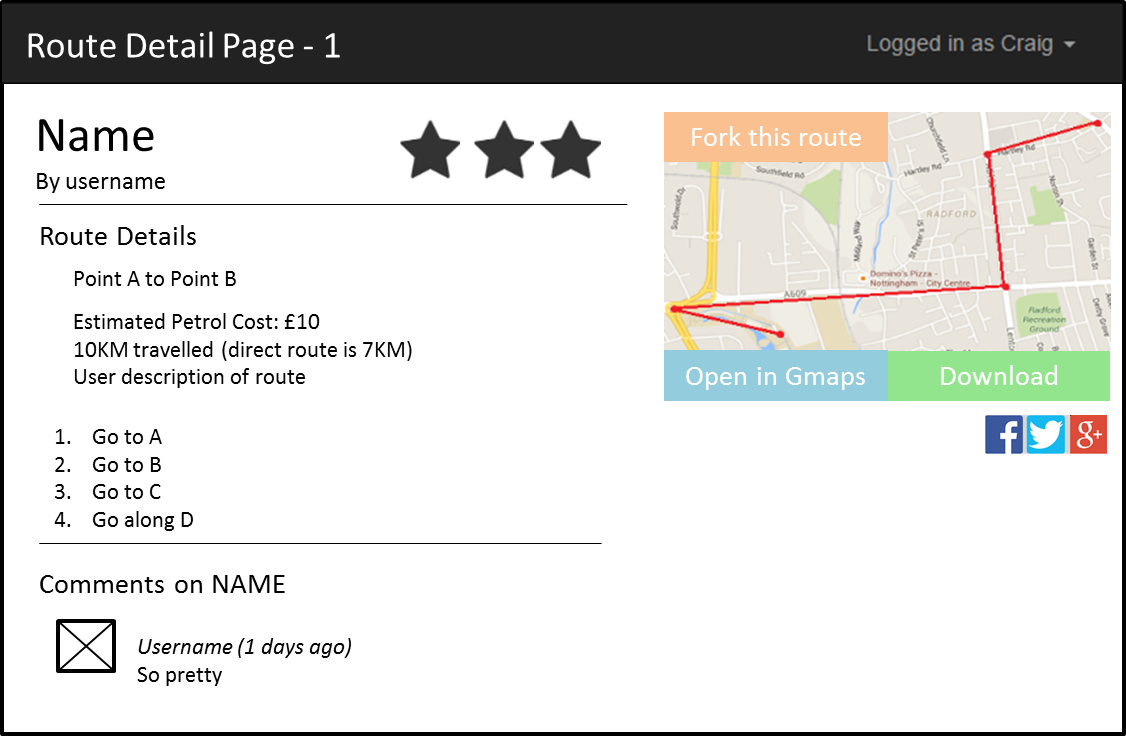
\includegraphics[width=0.5\textwidth]{images/ui-detail-1.png}
	\end{center}
	\vspace{-6mm}
\end{figure}

\paragraph{Two Column Design}\ \\
The second design also uses a two column layout, but utilises the space better. The map and it's details are on the left, so that users can see what they will be doing and where they will be going. If they are interested in the route, they can look to the right to see all the other information, as well as comments from other users. This prevents the user from being overwhelmed by too much information, but allows them to discover more if they wish.
\begin{figure}[!ht]
	\begin{center}
		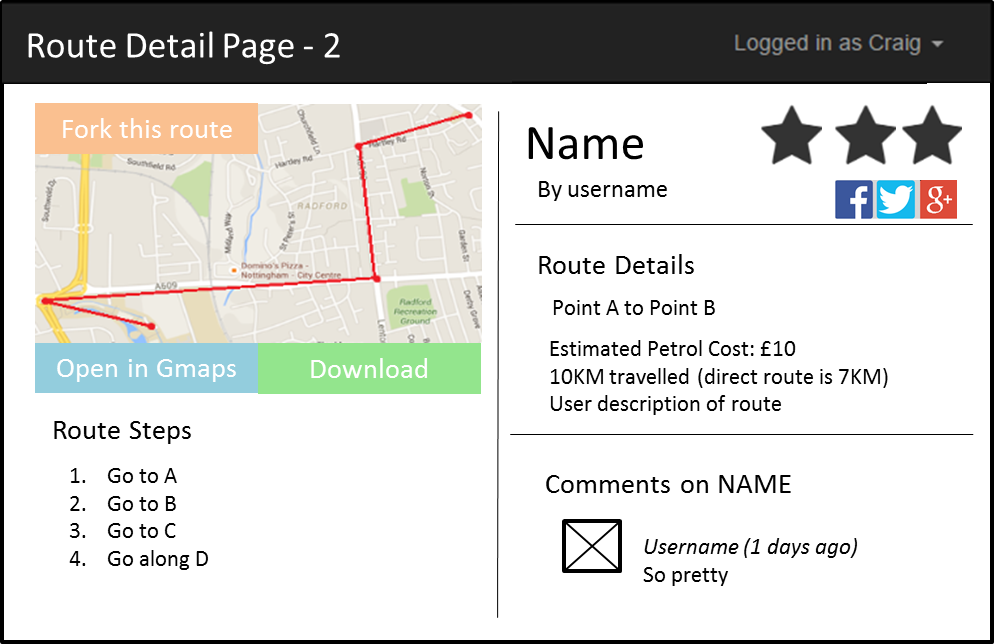
\includegraphics[width=0.5\textwidth]{images/ui-detail-2.png}
	\end{center}
	\vspace{-12mm}
\end{figure}


\newpage 
\paragraph{Map Centric Design}\ \\
The final design for the route detail page was very much focused on the visualization of the route. The only information displayed on the page was the name and rating of the map, and the route itself. The use could click on individual points on the route to get information about it (like a description and how long into the journey this point is). If they wished to see details about the route itself, there was a button for this on the side, which would bring up a side-bar element contain this information. They could also click the ``See comments'', and ``Fork this route'' buttons to display those features in the sidebar. This is a clean, minimalistic design, but could have issues with where users may not know how to see key route information and other user's comments.
\begin{figure}[!ht]
	\begin{center}
		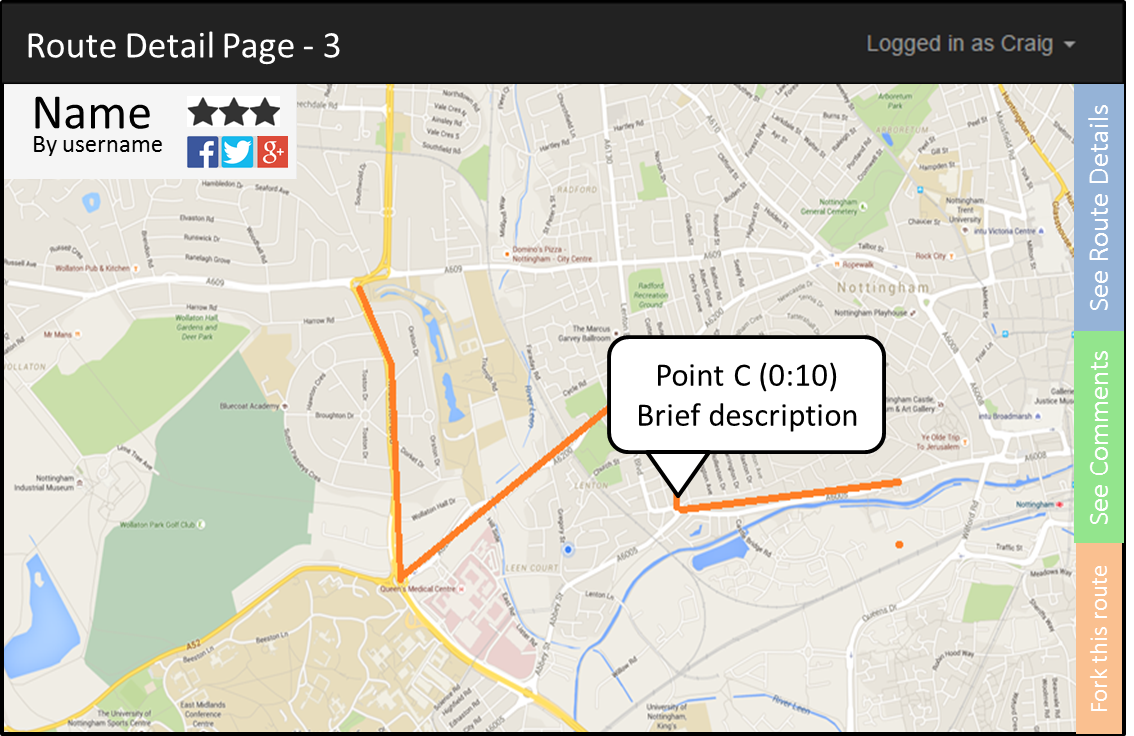
\includegraphics[width=0.7\textwidth]{images/ui-detail-3.png}
	\end{center}
	\vspace{-6mm}
\end{figure}

\subsection{The Route Creation Page (RCP)}
The route creation page was used to specify points of interest, and combine them into a route. The user can use a map to click on locations to add them as points of interest, and they will be automatically connected. The user is free to add points, delete points, and edit the order of points as they wish. Once the route is complete, the user can submit it, allowing them to specify a name, the privacy settings, and a description (FR 2, 2.1, 2.2, 8).


\begin{figure}[!ht]
\centering
	\begin{minipage}{.49\textwidth}
		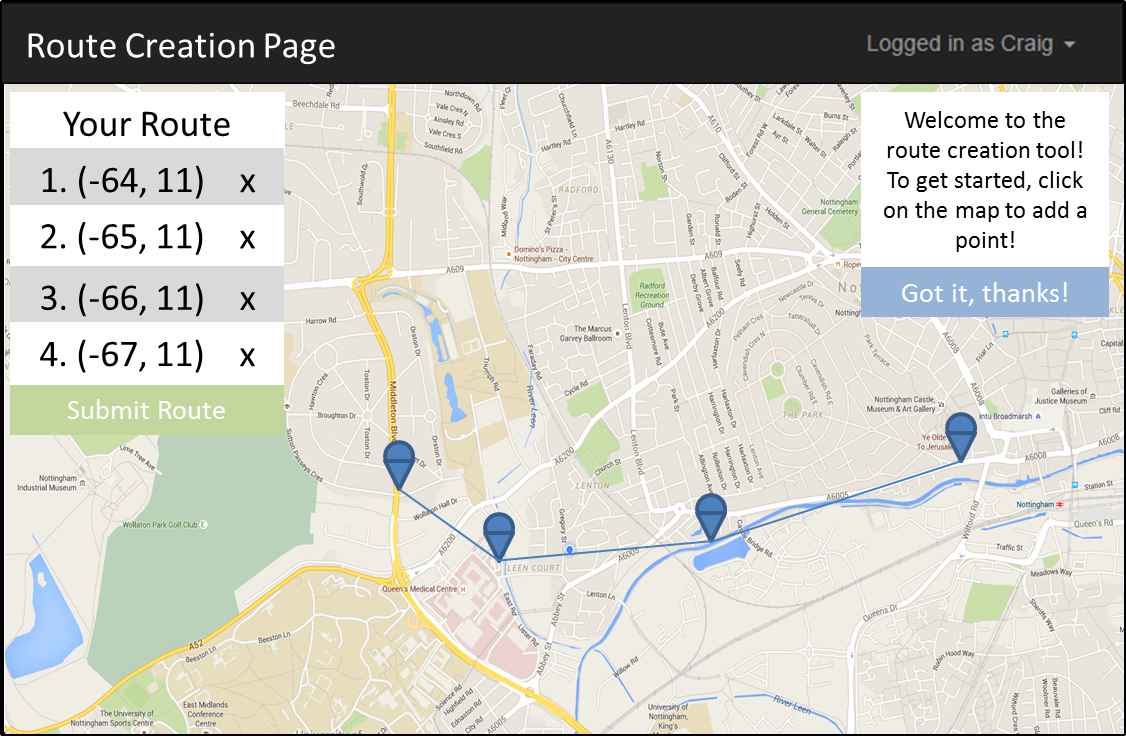
\includegraphics[width=0.99\textwidth]{images/ui-rcp-1.png}
	\end{minipage}
	\begin{minipage}{.49\textwidth}
	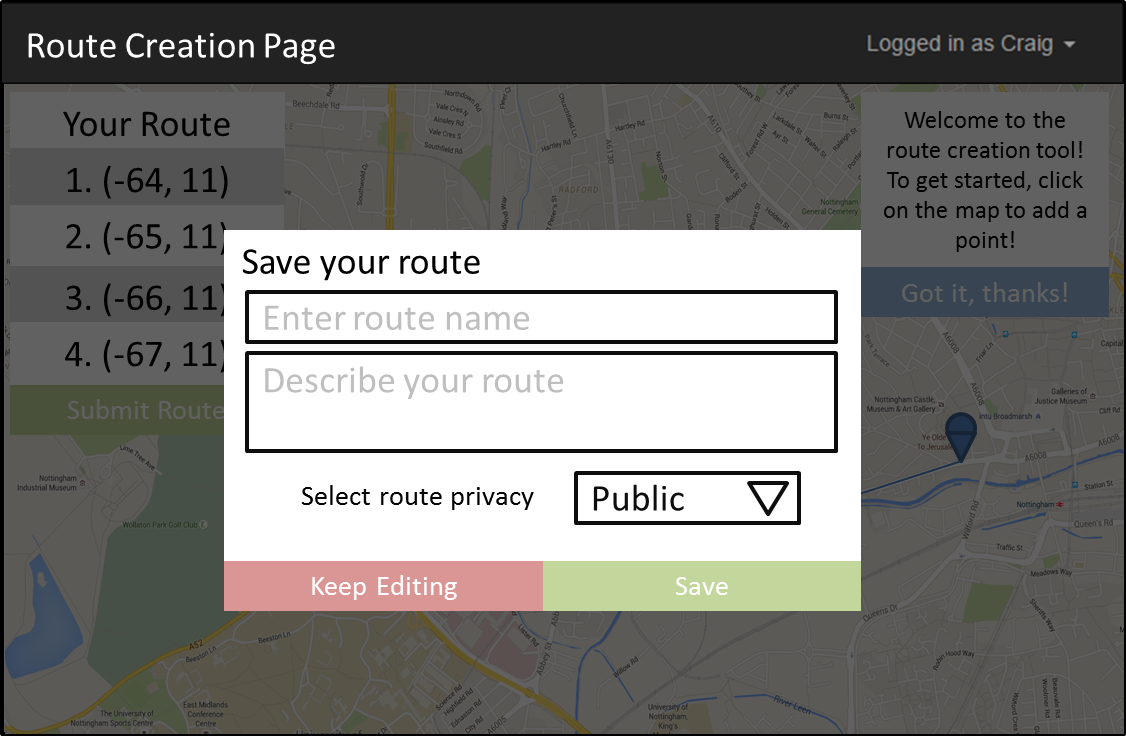
\includegraphics[width=0.99\textwidth]{images/ui-rcp-2.png}

	\end{minipage}
\end{figure}


\newpage 
\subsection{Generic Page Designs}
\label{subsec:gpd}
This section details the ``generic'' pages of the application - those that are mostly form based, and do not require a large amount of design consideration. It includes a basic design, annotated with the functional requirements of the system. 


\subsubsection{Login Page}
The login page is as simple as possible, as to not detract from the purpose of the page. It provides the ability to log in to the user's account (FR 9), by entering their username and password, and the ability to go to the sign up page, if they do not have an account (FR 4). There will be a large scenic picture in the background, as this will increase the aesthetic of the page, fit with the team of the application, and hopefully trigger some emotional response from the user.
\begin{figure}[!ht]
	\begin{center}
		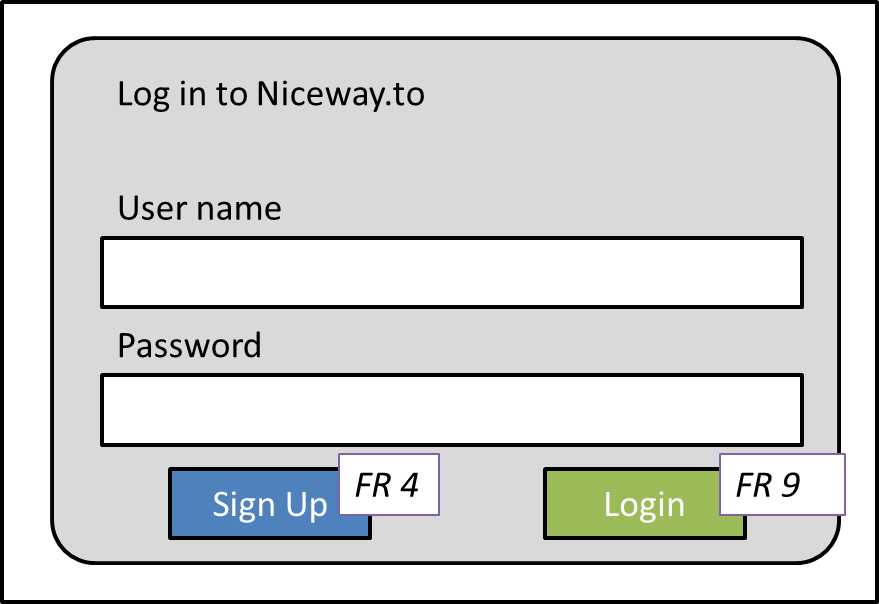
\includegraphics[width=0.45\textwidth]{images/ui-login.png}
	\end{center}
	\vspace{-6mm}
\end{figure}

\subsubsection{Sign Up Page}
Almost exactly like the login page, the sign up page is a very simple form allowing for users to enter in their details and create an account (FR 4), without being distracted by others elements on the page. This will actually be present on the same page as the login page, so the user is not required to navigate to another page simply to sign up, instead they can do it from the log in page, which will speed of the process of creating their account.
\begin{figure}[!ht]
	\begin{center}
		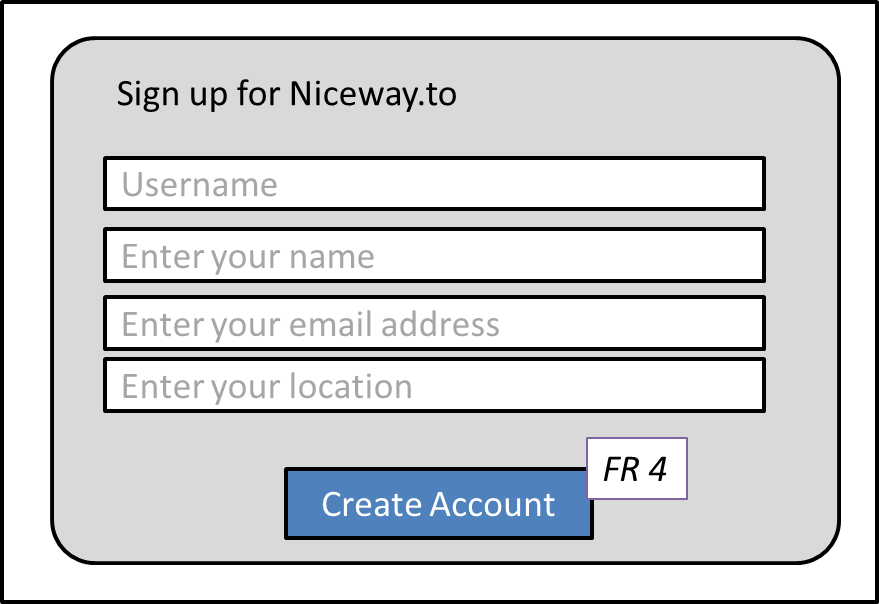
\includegraphics[width=0.45\textwidth]{images/ui-signup.png}
	\end{center}
	\vspace{-6mm}
\end{figure}

\newpage 
\subsubsection{Account Page - My Routes}
The ``My Routes'' page is used to display and manage all of the routes that a user has submitted, or forked, with the ability to add a new route (FR 9.2, 2, 2.1, 2.2). It will be on a generic ``My Account'' page, which means all similar actions are clustered together, and the user will know exactly where to navigate to perform any given task. On this particular page, the user's routes will be listed, along with key information (name, start location, end location, and privacy), with the ability to edit these settings, edit the route, delete the route, or export/download the route (FR 6). For users with many routes, a paginated view will be displayed.
\begin{figure}[!ht]
	\begin{center}
		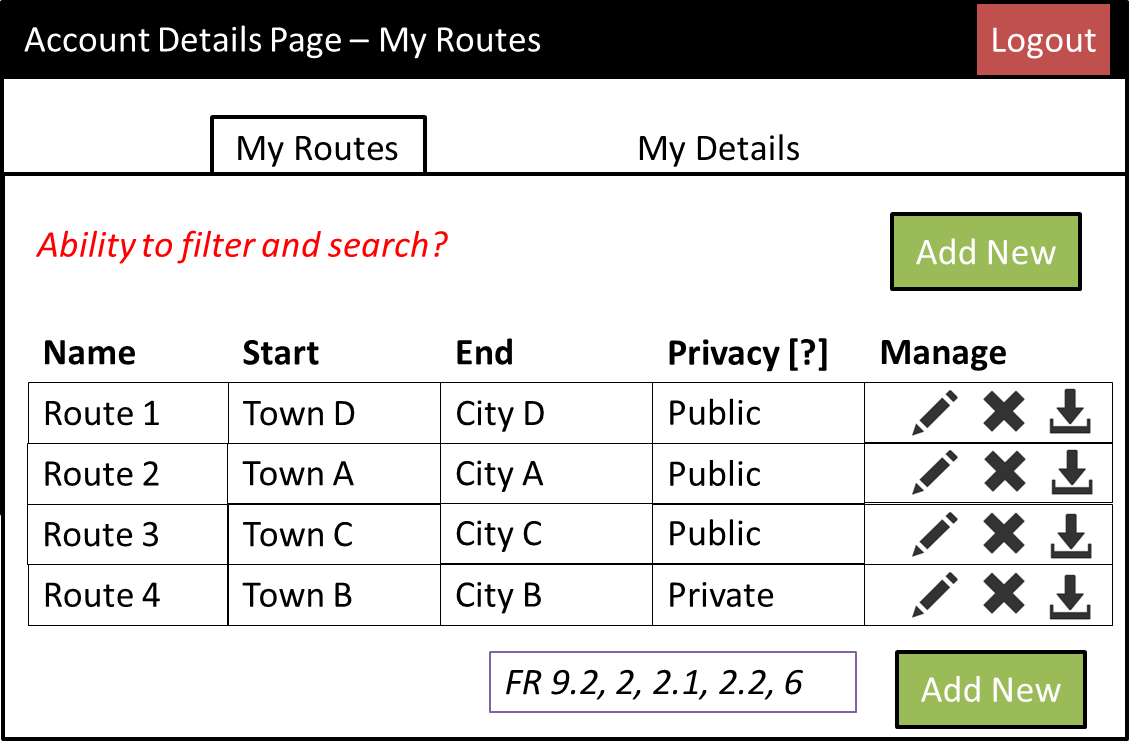
\includegraphics[width=0.6\textwidth]{images/ui-myroutes.png}
	\end{center}
	\vspace{-6mm}
\end{figure}\ \\

\subsubsection{Account Page - My Details}
Similarly to the ``My Routes'' page, the ``My Details'' page will be accessible from the generic ``My Account'' page. This page will simply display all of the user's data (excluding their password), with the ability to modify and update them (FR 4, 9.1). The page will be split into sections, so that similar data is situated together, for instance, the personal details section, and the update password section. This is so that users can jump to the exact functionality they require, rather than having to look through a large list of possible options. Users will also be given the ability to close their accounts on this page. 
\begin{figure}[!ht]
	\begin{center}
		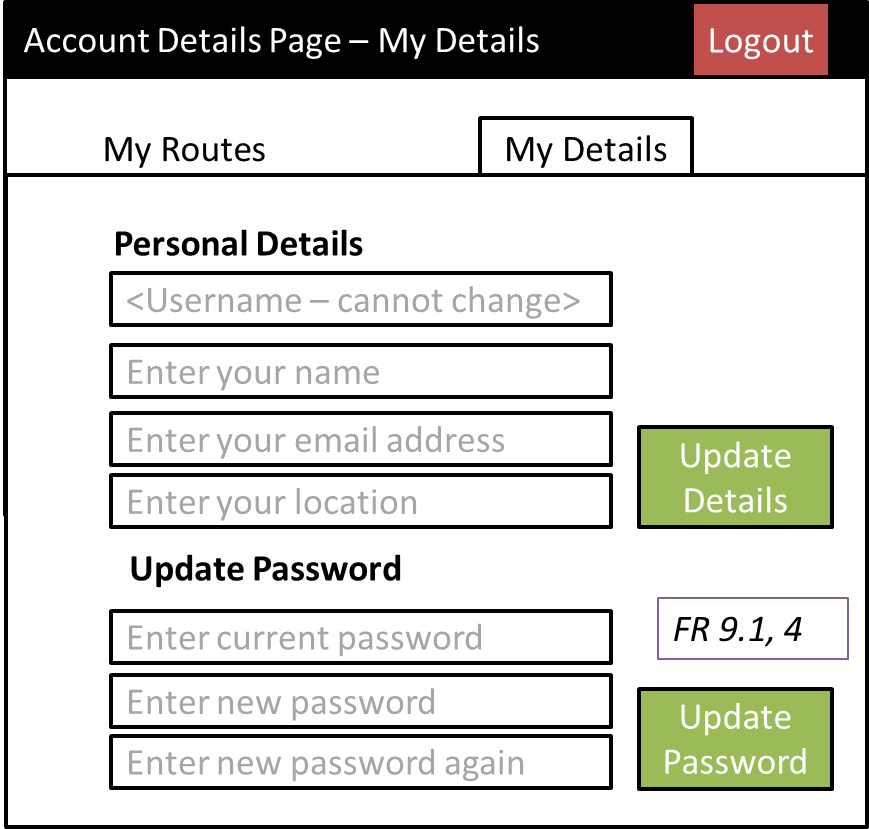
\includegraphics[width=0.5\textwidth]{images/ui-mydetails.png}
	\end{center}
	\vspace{-12mm}
\end{figure}

\subsubsection{Account Page - Administration}
The final generic page is the administration page, which like the previous two pages, will be located in the generic ``My Account'' page. This page will only be viewable and accessible to users with administrative privileges on Niceway.to. The page will provide multiple tools that the administrators can use to maintain the site, and manage users. The keys features are: a user search tool, with the ability to edit user details, delete users, ban them and shadow ban them \footnote{Allow the user to keep using the site, but none of their comments or routes will be visible to other users}; an account creation tool, with the ability to create new accounts on the site; an announcements tool, allowing the admin to post announcements to the site (as well as email users); and some server management tools, including making backups, reauthorizing active sessions, and locking the site. Similarly to the accounts page, these will be split up, so they are easier to see as distinct tools. 
\begin{figure}[!ht]
	\begin{center}
		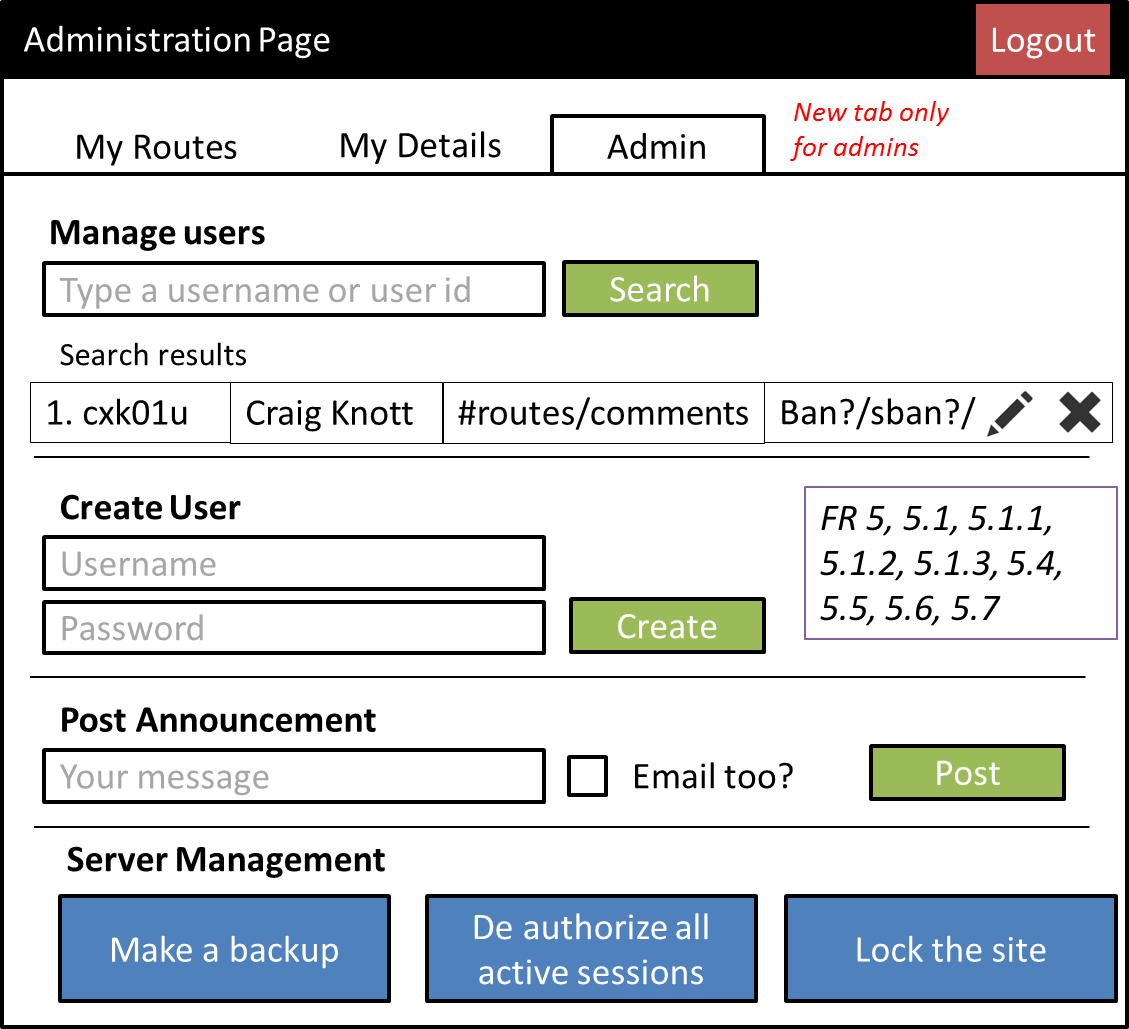
\includegraphics[width=0.7\textwidth]{images/ui-admin.png}
	\end{center}
	\vspace{-6mm}
\end{figure}


 
\subsection{User Flow Diagram}
 This diagram shows the expected user flow through the application. All user journey's will begin on the landing page, which also serves as the route discovery page. From here, users are free to search for routes, and experience the application, without every having the need to log in. They will have the ability to sign in, or sign up, from multiple locations, however, to increase the likelihood of them doing so (for instance, in the navigation bar of every page, and on the route detail page, prompting them to sign up so they can comment). Once a user has searched for a route, they will be taken to the route detail page, which will give users all the necessary information so that they can complete the route.\ \\
 \ \\
 If users wish to log in, or sign up, they will then be able to access their profile page, where they can see their submitted (and forked) routes, and modify their personal information. This is also where administrators will be able to access administrative tools for the management of the application. \ \\
 \ \\
The final feature available is route creator, which the user can access from the landing page (with the ``submit new route'' button), or from the ``My Routes'' section of the profile page. This means that it is extremely easy for the user to submit content to the site, as they are confronted with this option as soon as they visit the site, and whenever they view their other submissions.
 
 \begin{figure}[!ht]
 \begin{center}
 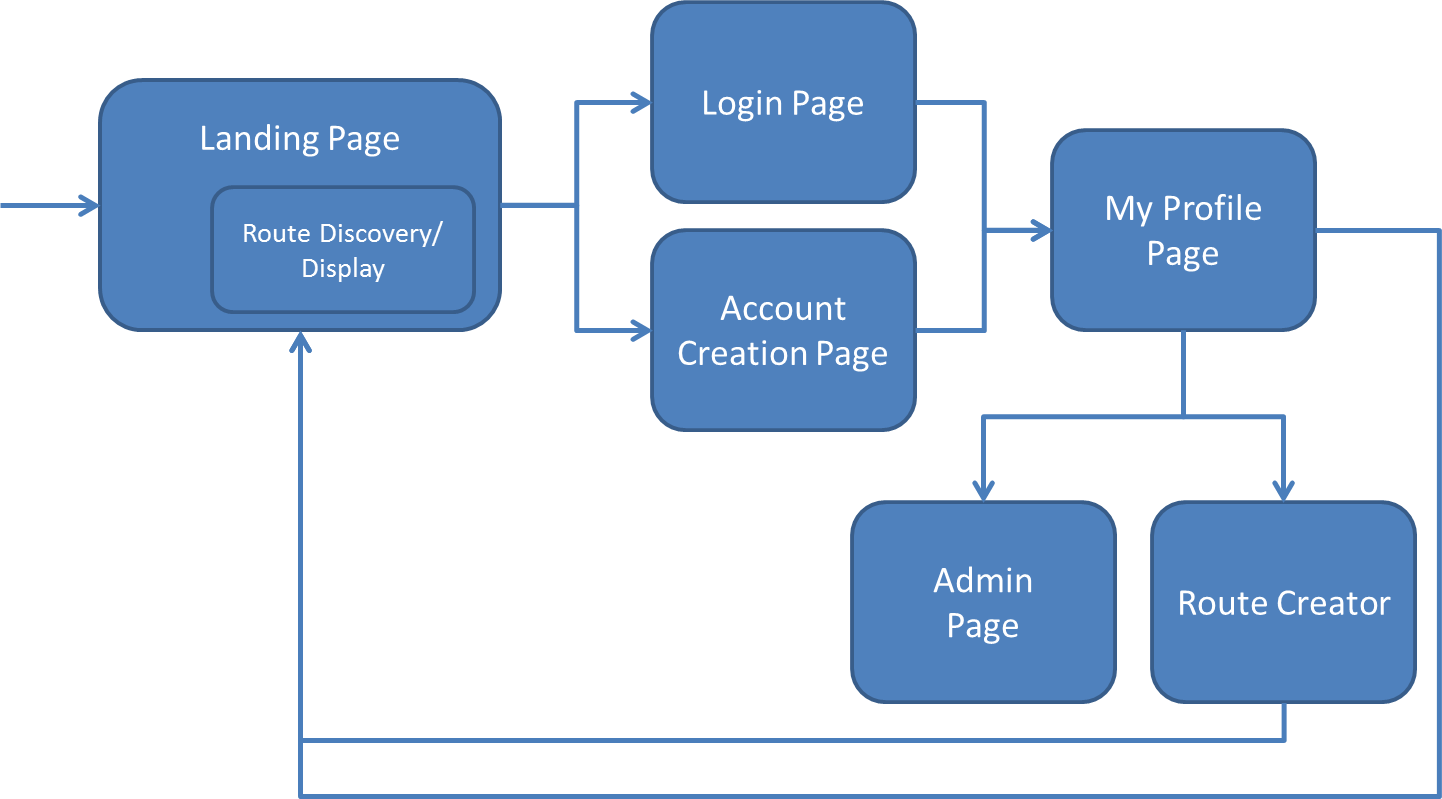
\includegraphics[width=0.7\textwidth]{images/flow.png}
 \end{center}
 \vspace{-6mm}
 \end{figure}

\section{Market Research}
\subsection{Analysis Of Similar Applications}
In this section, some other applications that are similar will be investigated, specifically mapping applications that either lets users submit their own routes, or allows for the browsing of scenic routes. The three tools that were investigated were Google's ``My Maps'' tool, a website called My Scenic Drives, and MADMAPS. The advantages and disadvantages of each were discussed, and the features that would be useful additions to Niceway.to were highlighted.

\paragraph{Google's ``My Maps'', \url{https://www.google.com/maps/d}}\ \\
Google Maps offers you the ability to plot maps and save them to your Google account, in order to access them later. It also allows you to share those routes with others via various social media. It has many features that would be useful in Niceway.to, including: a graphical tool for visualising the route, the ability to modify the route from this graphical interface, the ability to add photos and videos to a specific waypoint, and the previously mentioned ability to share maps through social media. Another significant feature is that the tool allows you to plot all the points on the map, and then generate the route afterwards, which would be ideal for the Niceway.to implementation. The main problems with this tool are that it's very slow (requiring long loads between actions), it is not very intuitive to use (due to difficulty navigating), and it's not very well known (the route planning and sharing functionality, not Google Maps itself). The key difference between this tool and Niceway.to, is that it has no focus on scenic routes. Users are free to enter in a scenic route, but they are also free to share any regular route, which is not the purpose of Niceway.to. It is also more difficult to share these routes with the wider community, because the only sharing option is to social media, which means people you do not have on your social media will, in likelihood, never find your recommended route. This is a field in which Niceway.to would succeed, as there will be a specific tool for searching for routes, and a community will grow around the application. 

\begin{figure}[!ht]
\begin{center}
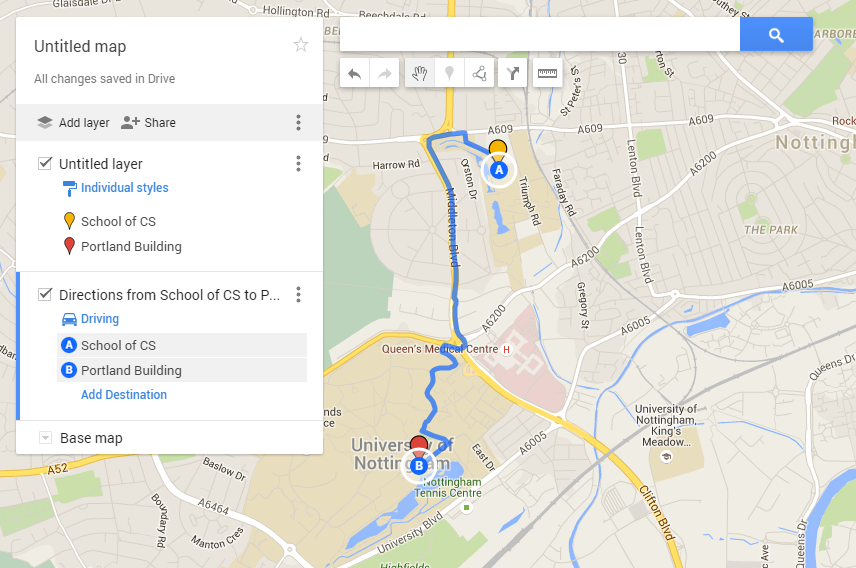
\includegraphics[width=0.7\textwidth]{images/google_maps.png}
\end{center}
\vspace{-6mm}
\caption{Google Maps ``My Maps'' route editing feature}
\vspace{-6mm}
\end{figure}

\paragraph{MyScenicDrives, \url{https://www.myscenicdrives.com}}\ \\
MyScenicDrives is a website that allows users to search for scenic routes by city, state or zip code (currently the service is only available in the United States), and view extremely detailed information about these routes (most routes come accompanied with a very lengthy description). This search functionality is similar to what is required by Niceway.to, but too primitive. MyScenicDrives gives the user no option to specify the start point or end point of a route, instead only allowing them to specify a general area in which the route takes place. For repetitive journeys for which the user knows the start and end points, but wishes to make more enjoyable, this tool would not be useful. This brings me onto another large issue with MyScenicDrives. It has a very small user base, which leads to a low number of available routes. For the majority of states, there were approximately five different routes, meaning there are only 250 or so for the entirety of the United States - a minuscule number. In all probability, this is due to the, apparently required, long written description. This could serve as a deterrent for users wishing to submit a route (especially new users, or those with little computing knowledge). However, the page on which the details of the route are displayed has many features that could be utilised well in Niceway.to. Specifically, information such as good times of the year to visit this route, locations of service stations, related routes, and a relevant description. Including some, or all, of the above fields in Niceway.to would be a valuable way to add more rich content - but by making them optional, the application is more appealing to use. 

\begin{figure}[!ht]
\centering
	\begin{minipage}{.49\textwidth}
		\begin{center}
			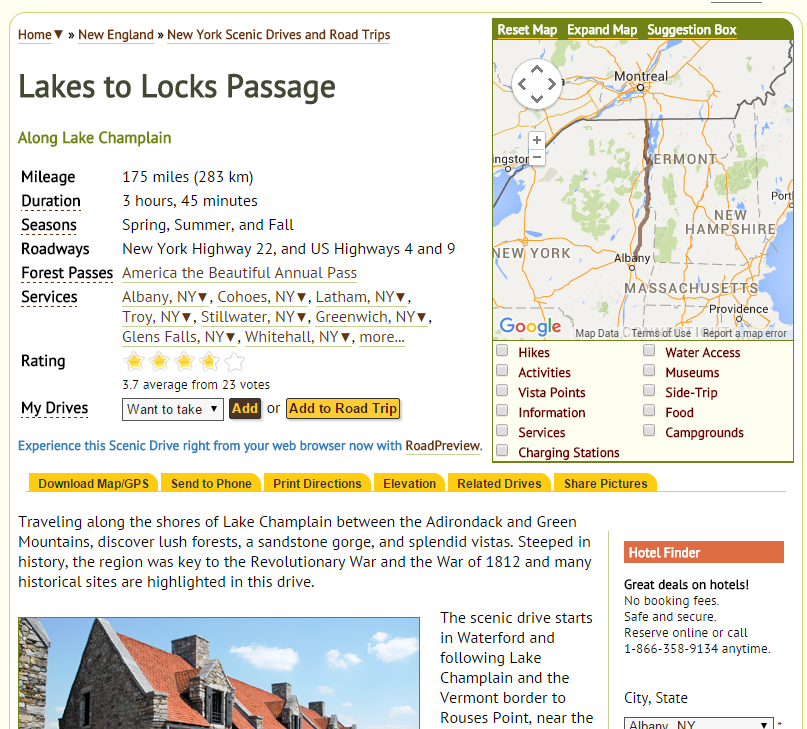
\includegraphics[width=0.9\textwidth]{images/msd-1.png}
			\caption{MyScenicDrive's Route detail page}
		\end{center}
	\end{minipage}
	\begin{minipage}{.49\textwidth}
		\begin{center}
			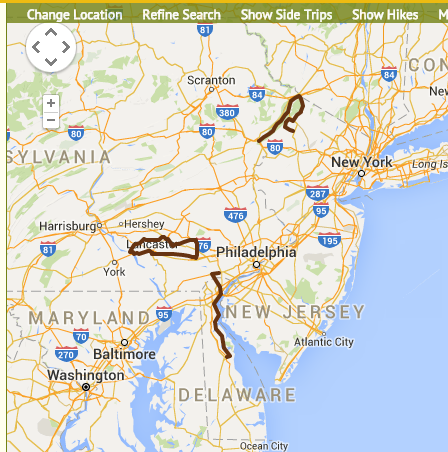
\includegraphics[width=0.8\textwidth]{images/msd-2.png}
			\caption{MyScenicDrive's Map Search Feature}
		\end{center}
	\end{minipage}
	\vspace{-10mm}
\end{figure}

\newpage 
\paragraph{Mad Maps}\ \\
The final mapping website that was investigated was Mad Maps, which, although aimed mostly at Motorcycle journeys, is a website which allowed you to purchase physical maps detailing scenic routes to travel, or view them on their mobile phone application. Immediately, the biggest down fall of this service was the cost. All the physical maps cost money, and you cannot preview them before purchasing. This is a big investment for something that the user may not enjoy, and could easily deter them from using this service. The routes on the mobile application are cheaper, and also more convenient, as they are in a digital format, but some can sell for as much as \$10, which again is a large sum of money to spend on something you may not enjoy. This service differs from Niceway.to in that users cannot submit routes in any way. Instead, the routes are compiled by ``experts'', which means there is no social aspect to generating routes, and the number of routes would be less than in a collaborative application. A user can submit photos to one of the designated points of interest along a route, and share it on Facebook, but there are social interactions within the application. One useful feature, however, is the ability to download the route to your phone, in case of internet connection failure. This could be utilised in Niceway.to, by allowing the user to load the route while they have internet, or save the route to their phone, and allow offline ``playback''. 

\begin{figure}[!ht]
\centering
	\begin{minipage}{.49\textwidth}
		\begin{center}
			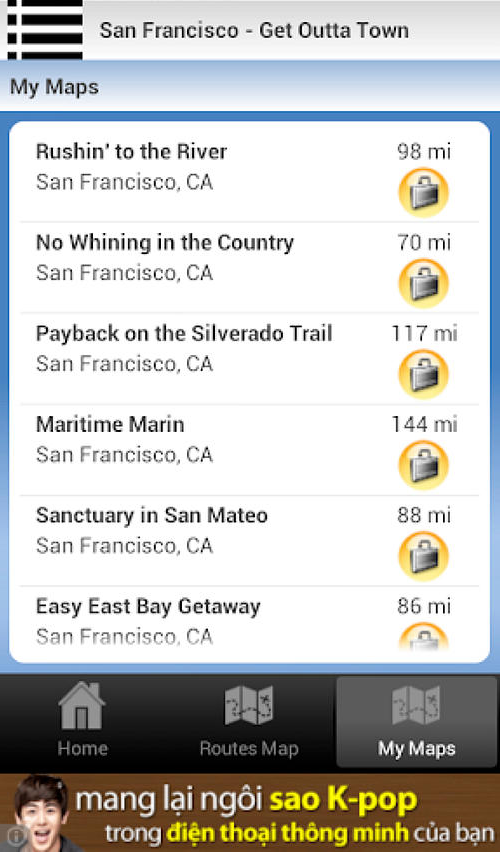
\includegraphics[width=0.5\textwidth]{images/mm-1.png}
			\caption{MAD MAPS' Route Listing Page}
		\end{center}
	\end{minipage}
	\begin{minipage}{.49\textwidth}
		\begin{center}
			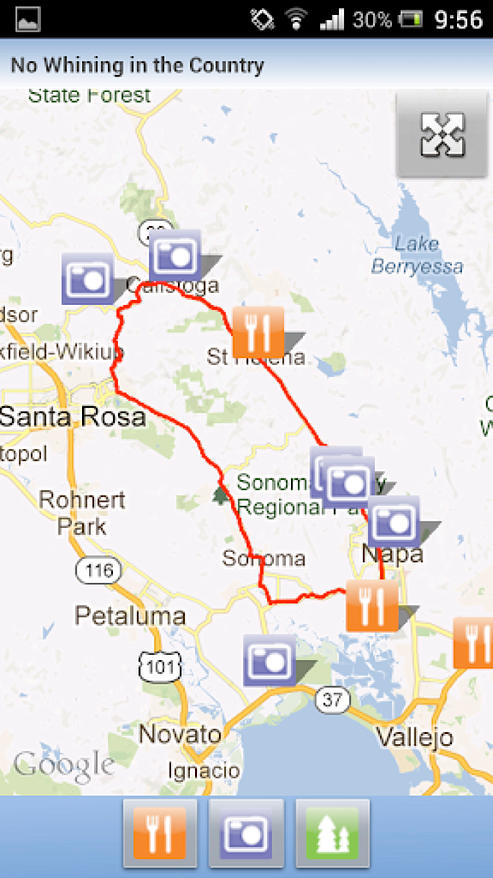
\includegraphics[width=0.475\textwidth]{images/mm-2.png}
			\caption{MADMAPS' Route Display Page}
		\end{center}
	\end{minipage}
\end{figure}

\subsection{Web Applications VS Native Mobile Applications}
It is important to decide the format of this kind of application, as this can have a huge effect on how well it is received by the market. In this section, the advantages and disadvantages of two possible approaches to the development of Niceway.to are discussed: as a web application, or as a native mobile application.

\paragraph{Web Applications}\ \\
Web applications are easy to write and don't require knowledge of a specialized language, as the front end is in HTML, CSS and JavaScript, and the backend can be whichever language the programmer is most comfortable with. As they are hosted on the internet, there is no need for the user to download them, which is something that sometimes puts people off from using a service, this also means that if the application is updated, they don't need to install any updates, and can get straight back to using the application. Web applications don't require any approval before being distributed, as they don't need to be put on an app store, and as soon as they are up, they are available to everyone, regardless of their device (unlike mobile apps, which generally target one specific operating system). \ \\
\ \\
However, not being available on an app store means it's more difficult to discover the application. Native applications are all visible within the market place, which is a lot smaller than the entirety of the world wide web. Another negative of web applications is that they require an internet connection to access (as they are web based), and they cannot fully utilise the native technology of the device they are on (unlike mobile apps which can access all the hardware of the phone they are on). However, web application advertisements are generally less intrusive than mobile ones, so running the application for free is much easier.

\paragraph{Native Mobile Applications}\ \\
Native mobile applications are good because they allow for greater exposure, as they have to be distributed through the app market place. This means there is a centralised place that your application will always be advertised on (although there is a negative that the application has to be submitted to the app store, and may require modifications to get it accepted, which could waste valuable time). This allows for multiple pricing models, a payment for downloading the app (which is less appealing for the user), or for free, with adverts (better, but sometimes the adverts can be very intrusive), or a free version, with the option to upgrade to remove adverts (best of both worlds). Native mobile applications can also be used offline, as they (generally) download all the content onto the user's phone, so it can be accessed regardless of internet connection (this however, is not really applicable to this project, because of the nature of it). This does mean, however, that the app needs to be downloaded (which is generally accepted nowadays, but could also lead to the app being ignored if the user, for instance, doesn't have enough space to download it), and any further updates to the application would need to be downloaded as well. While the application can utilise all the phone's native technology, it is only available for the platform that it was designed for (unless a tool to convert it is used, but this generally produces poor quality products). 
\input{sections/finaldesigns}
 \section{Final Designs}
 After the initial designs were created, they were shared with the client for feedback. This section summarises that feedback, as well as displays the new designs which will be used when implementing the system. This includes one single design for each of the main pages, and updated designs for the generic pages.\ \\
 \ \\
 The client's main comment was ``we see social commentary being relegated to a minimal part of the UI, something we believe should be addressed as the social component is key to the success of the project. The revised designs should feature the social commentary more prominently and also aim to encourage users to contribute.''\ \\
 \ \\
 As a result of these comments, the main two alterations were made, were to add more prominent social commentary features on the route detail page, and to add an explanation of what the site does on the landing page.
 \newpage

\subsection{Landing Page}
For the landing page, I choose to use the minimalistic design. This, when coupled with the helpful popover explaining the features of the site, made it very accessible to new comers. They knew exactly what the purpose of the site was, and how to get started, and there were no unnecessary extras that would pose an obstacle for them.
 \begin{figure}[!ht]
 	\begin{center}
 		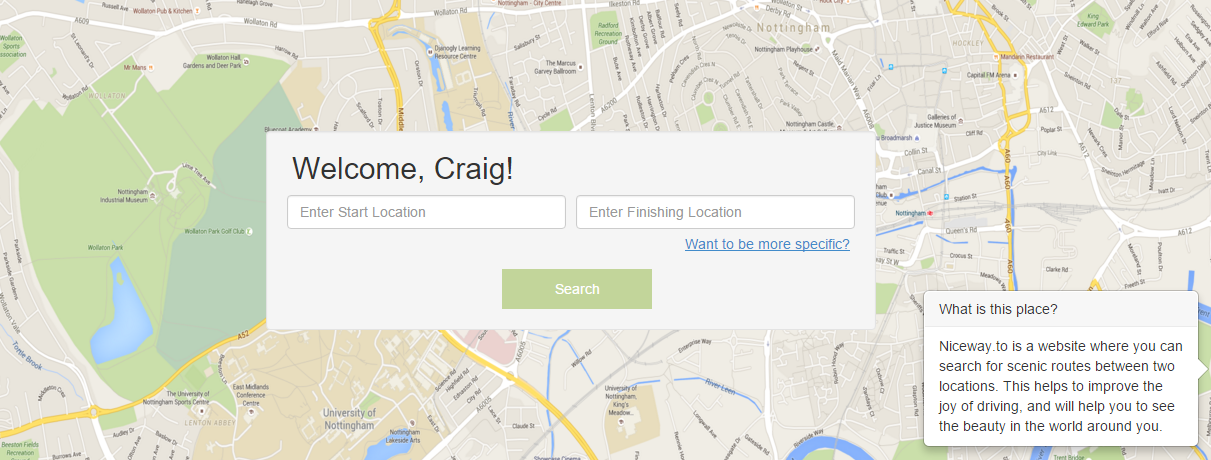
\includegraphics[width=0.9\textwidth]{images/final/landing.png}
 	\end{center}
 	\vspace{-6mm}
 \end{figure}
 
\subsection{Route Listing Page}
The final route listing page is a modification of the map-less initial design. The main change is to the ``Search Again'' feature. Instead of having the search at the top of the page, before the results, it is now on the left hand side. The advantage of this is that the user's are presented with all the search results instantly, instead of having to look down the page to find them, which could confuse them. Having the search terms present on the page is useful so that the user can see any mistakes, or easily modify their current search results.
 \begin{figure}[!ht]
 	\begin{center}
 		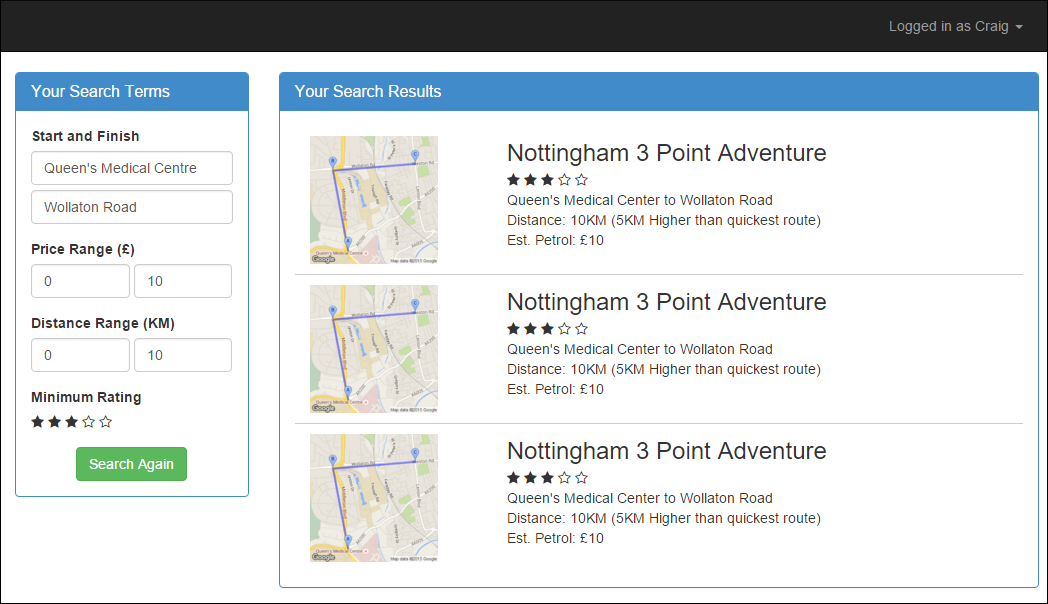
\includegraphics[width=0.9\textwidth]{images/final/listing.png}
 	\end{center}
 	\vspace{-6mm}
 \end{figure}

\newpage
\subsection{Route Detail Page}
The route detail page was the page that had the most changes between the initial and final designs. This was based off client feedback that the social interactions were not prominent enough. In light of this, the design was modified so that there were two columns: one for all the route details, and the other for only social commentary. This meant that the social aspect of the application was extremely prominent. The social stream was an amalgamation of all shares, comments, and fork that this route had received. The user will be able to filter this stream to only see content relevant to them. It also contains large social media share buttons, and a large comment box, with friendly prompts for the user to interact as well.
 \begin{figure}[!ht]
 	\begin{center}
 		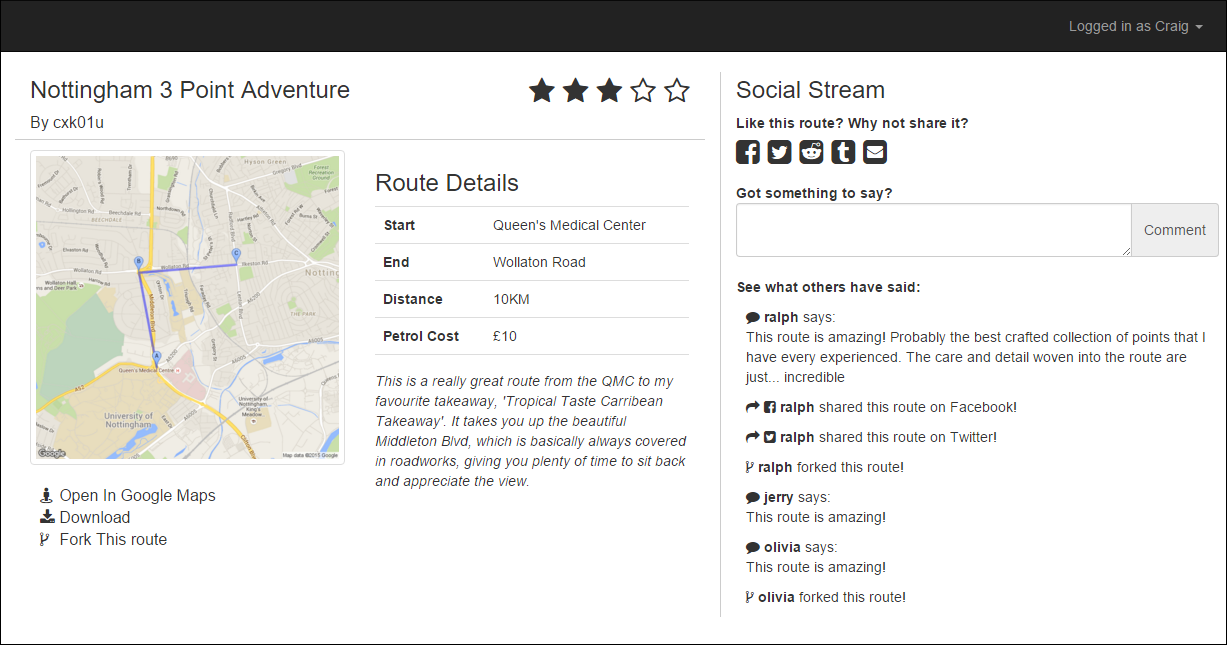
\includegraphics[width=0.9\textwidth]{images/final/detailpage.png}
 	\end{center}
 	\vspace{-10mm}
 \end{figure}


\subsection{Route Creation Page}
The purpose of the route creation page was to allow to user to seamlessly interact with the map, and plan their route. This design has a small explanation in the top right, so the users know what to do, but other than that, there is very little between the user and the map. In fact, the only UI element on the page is a small box on the left hand side, which gives a list of the points the user has already entered, so that they can reorder them, and delete them.

\begin{figure}[!ht]
	\begin{center}
		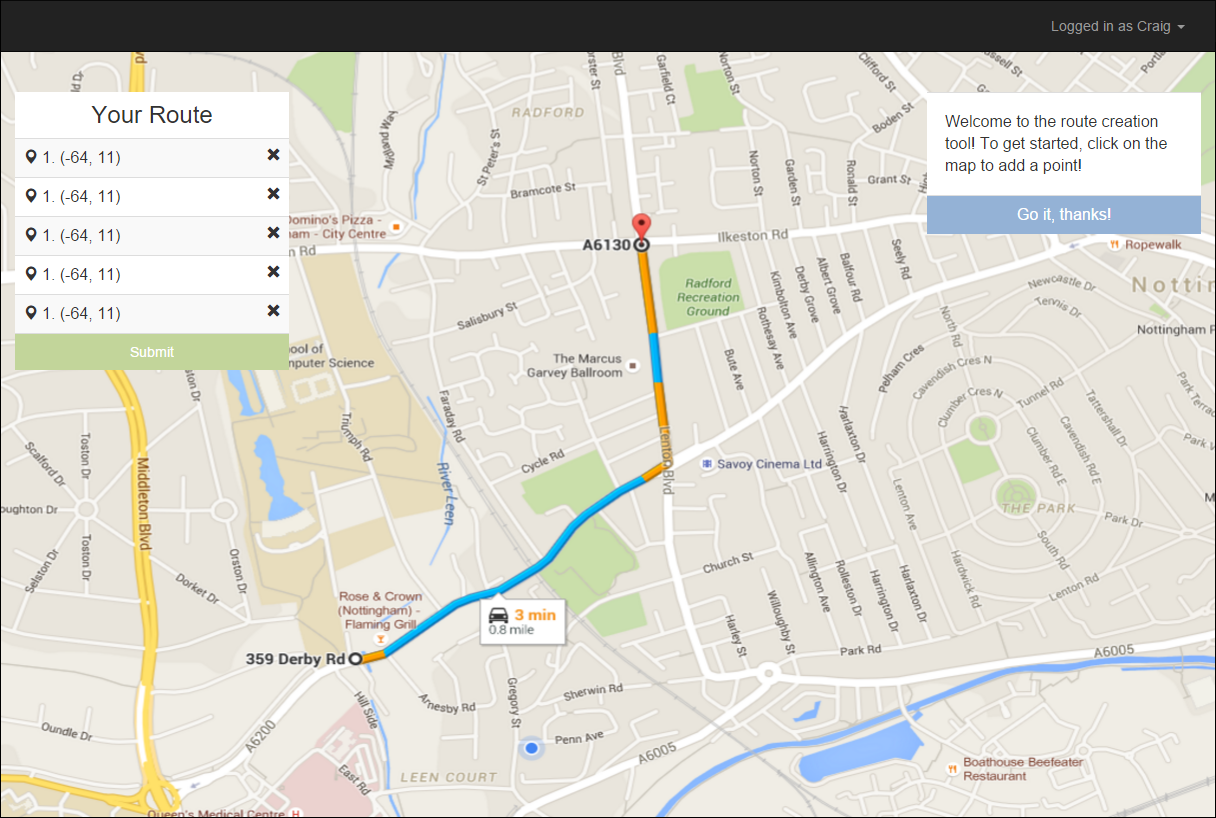
\includegraphics[width=0.7\textwidth]{images/final/creation.png}
	\end{center}
	\vspace{-16mm}
\end{figure} 
 
 
 \newpage
 
 
\subsection{My Details Page}
The ``My Details'' page was one of the three ``My Account'' pages that the users could potentially access. On the right, there is a small navigation menu, which directs to the other pages, as well as containing a brief description about each of those pages.\ \\
\ \\
The page itself is very simple. It lists all of the user's information in text entry fields. This means that modifying the information is extremely simple and intuitive, and users would not be confused as to the purpose of this page.

\begin{figure}[!ht]
	\begin{center}
		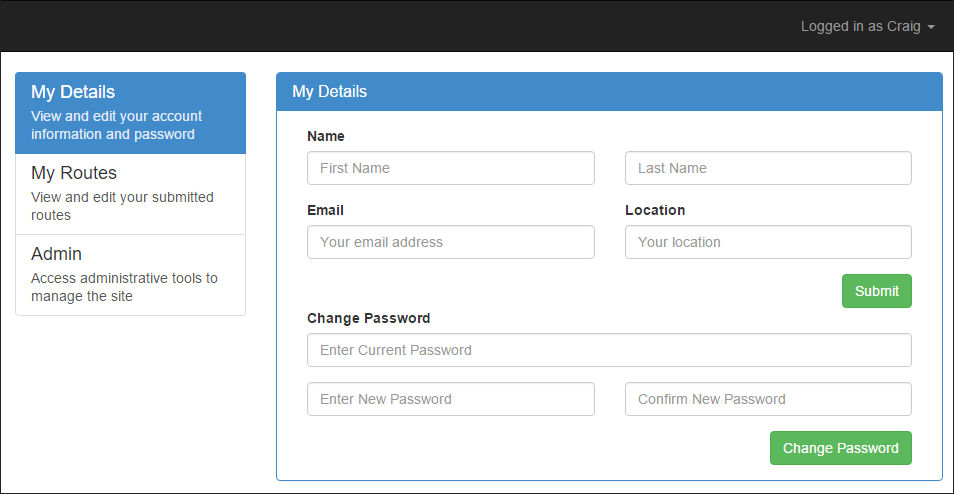
\includegraphics[width=0.8\textwidth]{images/final/mydetails.png}
	\end{center}
	\vspace{-6mm}
\end{figure}

\subsection{My Routes Page}
The ``My Routes'' page allowed users to see a list of all the routes that they had submitted. The could then do three things: edit the route (taking them to the route creation page), download the route, or delete the route (after asking if they were sure).\ \\
\ \\
Users also have the ability to add new routes from this page, which means this page can be considered the hub of all route activity. 

\begin{figure}[!ht]
	\begin{center}
		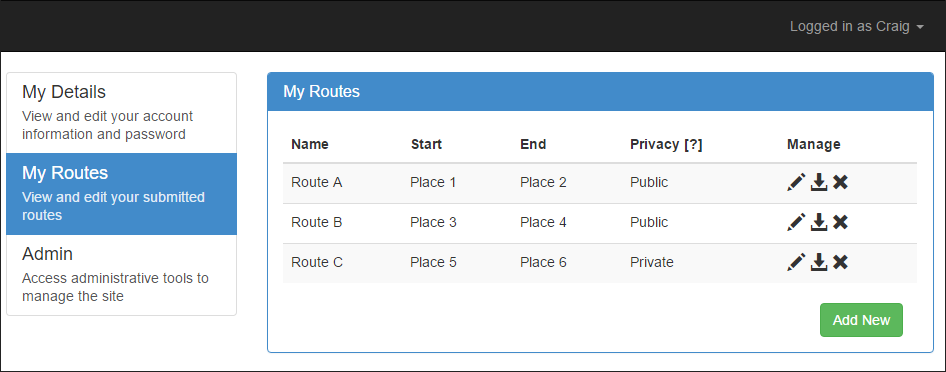
\includegraphics[width=0.8\textwidth]{images/final/myroutes.png}
	\end{center}
	\vspace{-6mm}
\end{figure} 
\newpage 

\subsection{Admin Page}
The admin page is only available to users that have been marked as the administrators of the application, which will stop regular users accessing these tools, and potentially causing harm to the application or its users. The page itself is used for the management and maintenance of the application. All the different tools are in separate panels, allowing the admins to clearly identify which tool they need to use, and allowing them to focus only on that part of the page. It features the ability to manage users, create users, post announcements, and manage the server, all from this control panel.

\begin{figure}[!ht]
	\begin{center}
		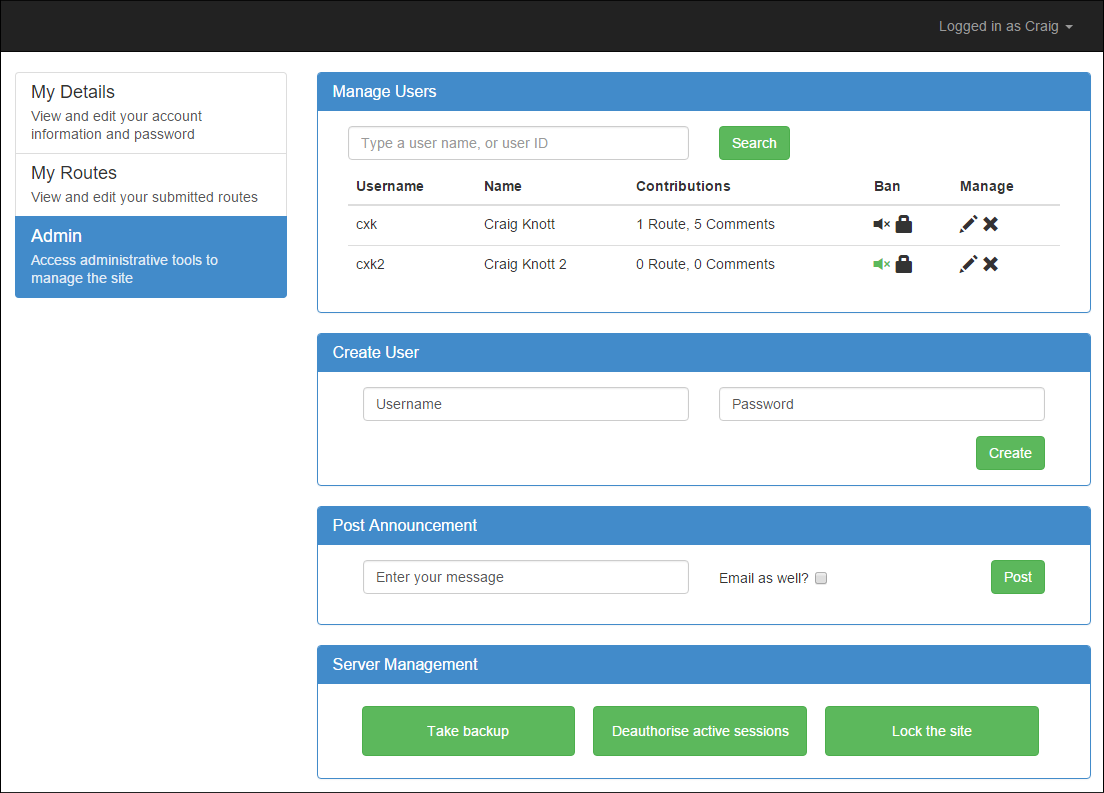
\includegraphics[width=0.7\textwidth]{images/final/admin.png}
	\end{center}
	\vspace{-6mm}
\end{figure} 

\subsection{Login Page}
The login page didn't change much between the initial and final designs, as it is a relatively simple page. The main change is moving the login, and signup buttons to separate lines and adding the ``or'' text. Originally they were both on one line, so it was less obvious which button needed to be pressed at a glance. With them on separate lines, the user would naturally look at the top button first - allowing them to login, which was the purpose of the page. If they didn't wish to log in, they would continue looking, and would identify the sign up button, which they could then click.

\begin{figure}[!ht]
	\begin{center}
		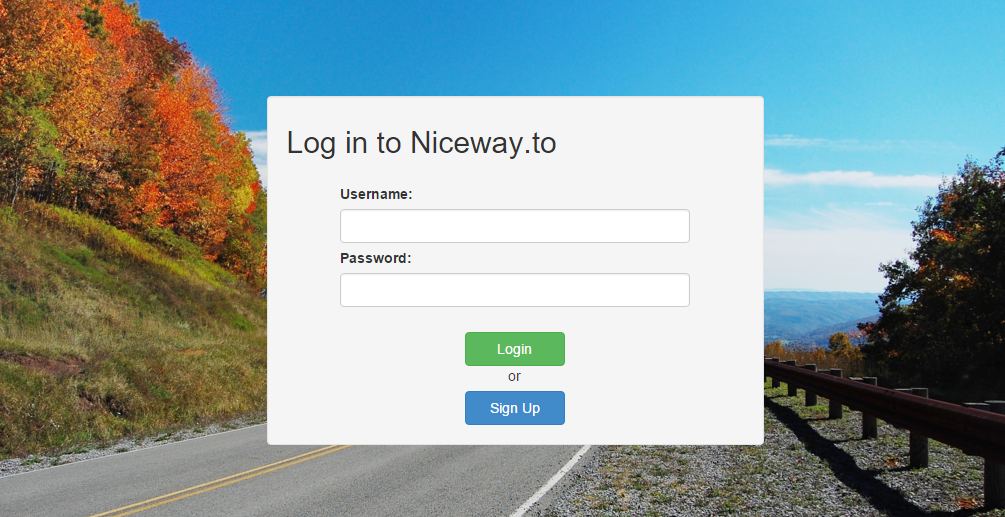
\includegraphics[width=0.7\textwidth]{images/final/login.png}
	\end{center}
	\vspace{-6mm}
\end{figure}

\subsection{Signup Page}
The final page was the signup page which, like the log in page, is very simple, and didn't require many changes between the initial version and the final version. The main difference was highlighting which fields were not required (by adding the optional text to them)m and allowing users to specify their passwords (which was not present on the initial designs by mistake).
\begin{figure}[!ht]
	\begin{center}
		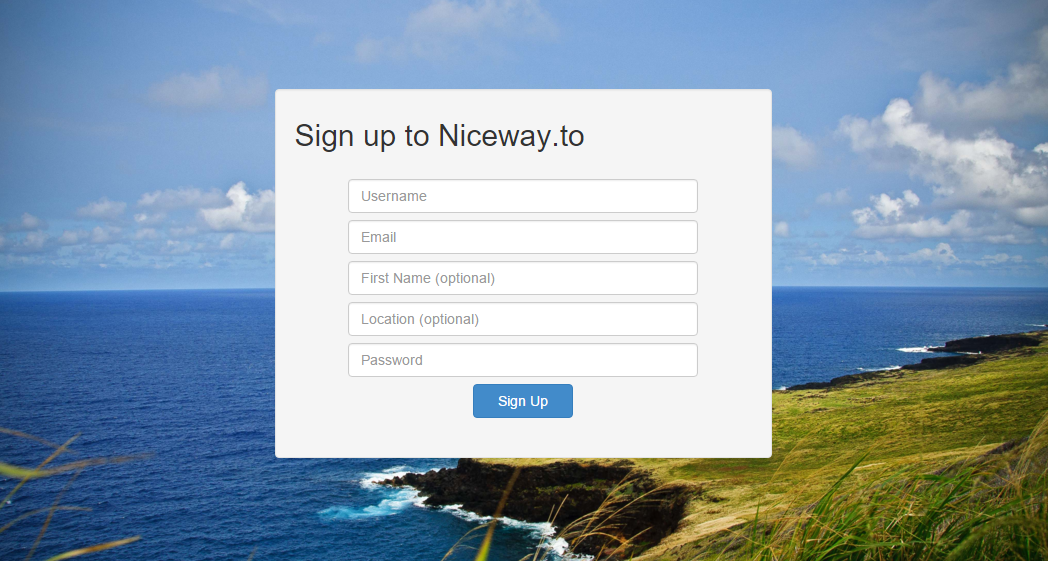
\includegraphics[width=0.7\textwidth]{images/final/signup.png}
	\end{center}
	\vspace{-6mm}
\end{figure}




 
 




 
  
 
  
\end{document}